
\begin{question}
Solve the system of equations.

\[\begin{aligned}
- 3 x^{2} + 6 x + y &= 28 \\
12 x - y &= -25
\end{aligned}\]
\end{question}

\begin{solution}
There is one solution.

\[(-1,13)\]

This system represents a parabola and a tangent line.

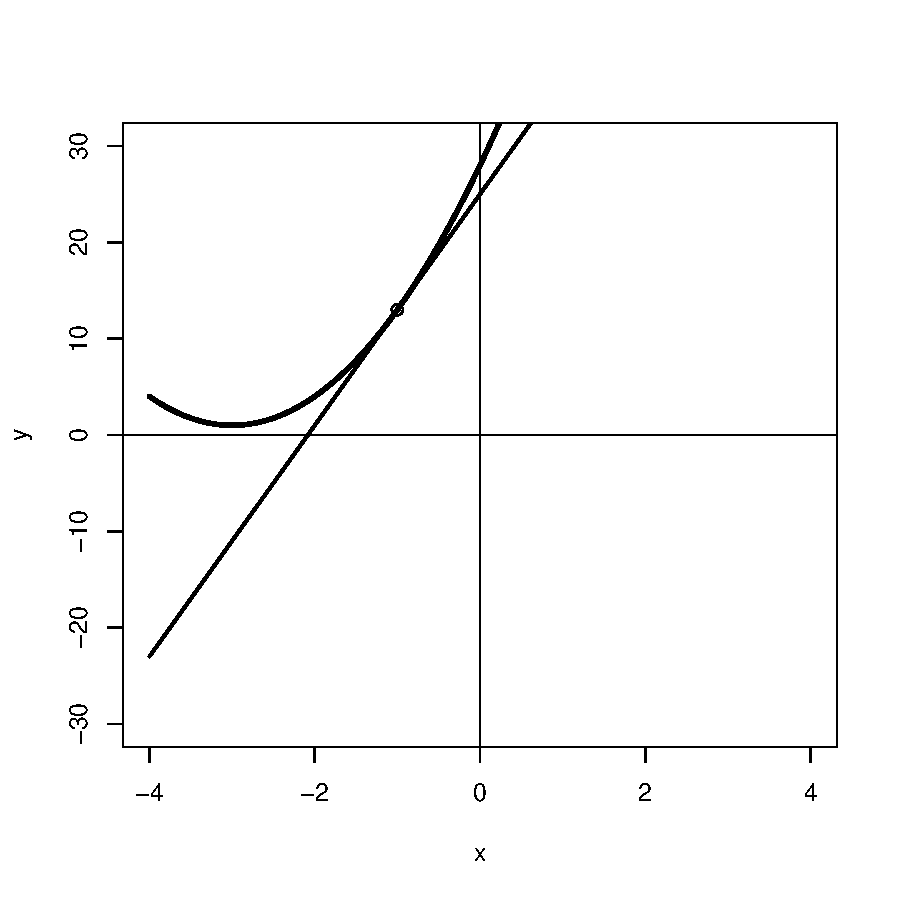
\includegraphics{unnamed-chunk-2-1-2.pdf}\\
\end{solution}

